\begin{frame}{Mechanics of Materials}
\protect\hypertarget{mechanics-of-materials}{}
Lecture 11 - Bending

Dr.~Nicholas Smith

Wichita State University, Department of Aerospace Engineering

22 September, 2020
\end{frame}

\begin{frame}{schedule}
\protect\hypertarget{schedule}{}
\begin{itemize}
\tightlist
\item
  22 Sep - Bending, Homework 4 Due, Homework 3 Self-Grade Due
\item
  24 Sep - Bending
\item
  29 Sep - Transverse Shear, Homework 5 Due, Homework 4 Self-Grade Due
\item
  1 Oct - Transverse Shear
\end{itemize}
\end{frame}

\begin{frame}{outline}
\protect\hypertarget{outline}{}
\begin{itemize}
\tightlist
\item
  shear and moment diagrams
\item
  graphical method
\item
  bending deformation
\item
  flexure formula
\end{itemize}
\end{frame}

\begin{frame}{shear and moment diagrams}
\protect\hypertarget{shear-and-moment-diagrams}{}
\begin{itemize}
\tightlist
\item
  The general approach to shear and moment diagrams is to first find the
  support reactions
\item
  Next we section the beam and instead of finding the internal force and
  moment at a single point, we find it as a function of \emph{x}
\item
  Many beams will require piecewise sectioning
\item
  We then draw this as a shear and moment diagram
\end{itemize}
\end{frame}

\begin{frame}{sign convention}
\protect\hypertarget{sign-convention}{}
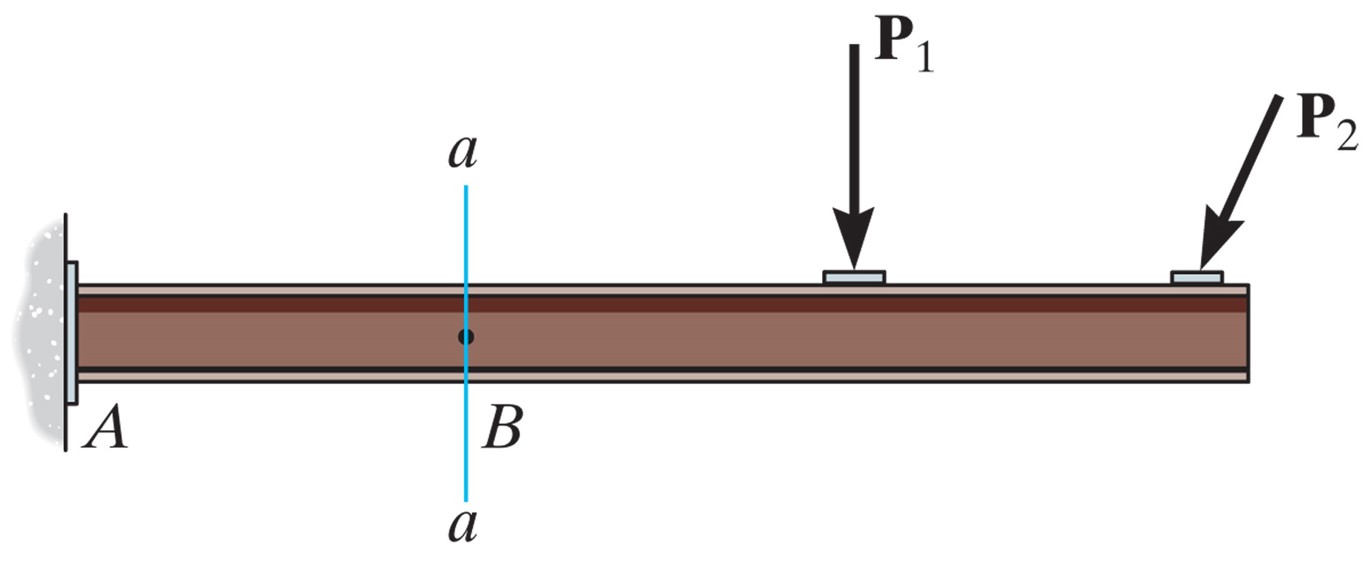
\includegraphics{../images/beam-internal.jpg}

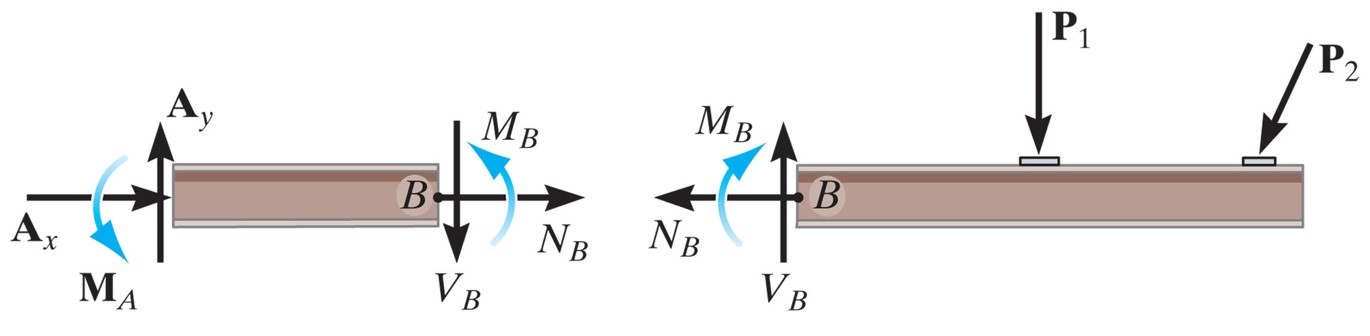
\includegraphics{../images/beam-internal-cut.jpg}
\end{frame}

\begin{frame}{example beam}
\protect\hypertarget{example-beam}{}
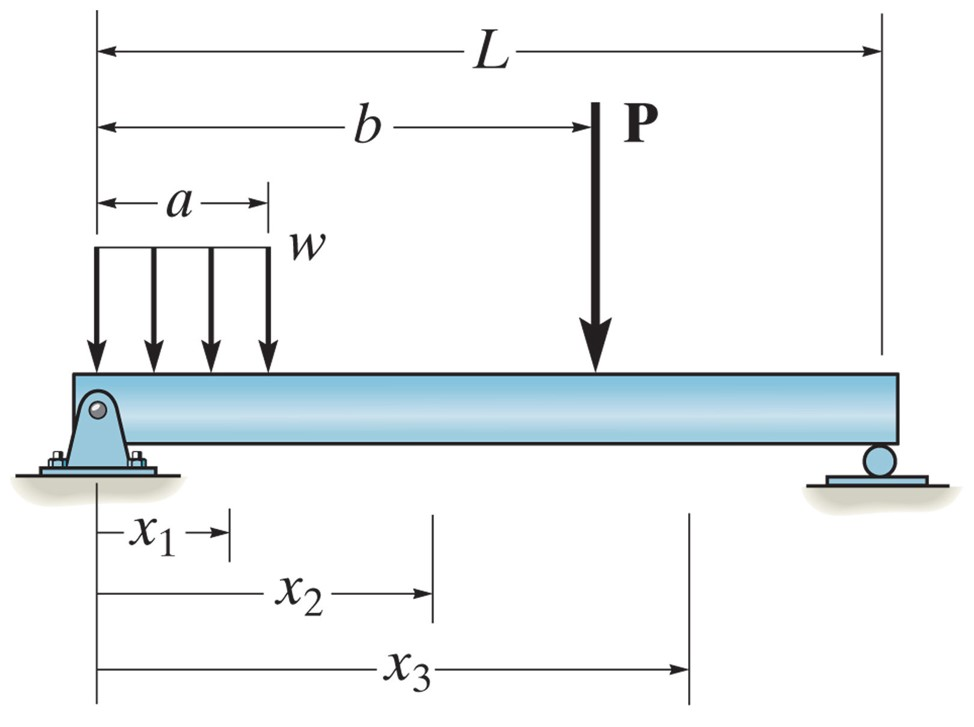
\includegraphics{../images/piece-wise-beam.jpg}
\end{frame}

\begin{frame}{example beam}
\protect\hypertarget{example-beam-1}{}
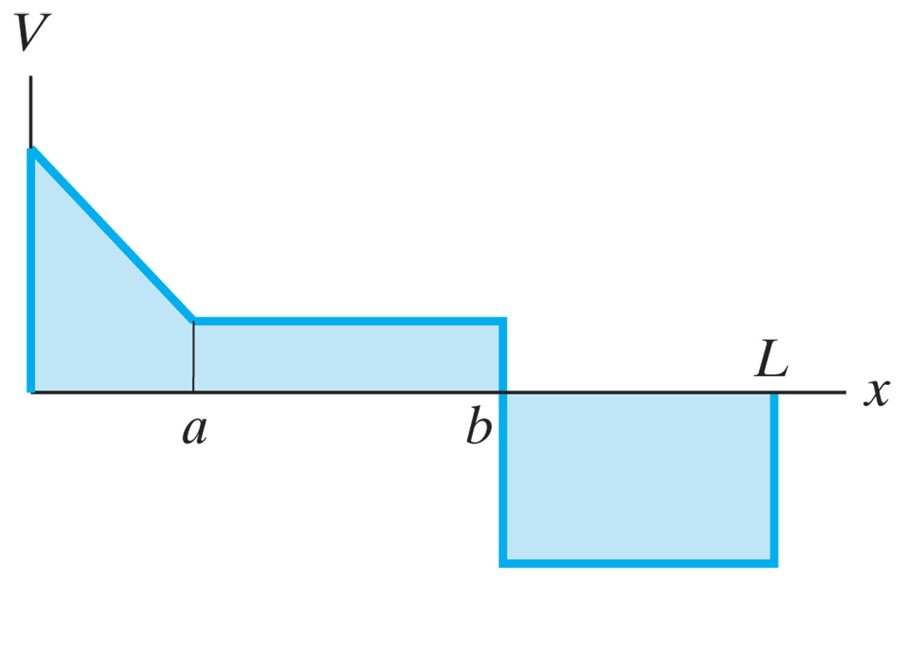
\includegraphics{../images/shear-diagram.jpg}
\end{frame}

\begin{frame}{example beam}
\protect\hypertarget{example-beam-2}{}
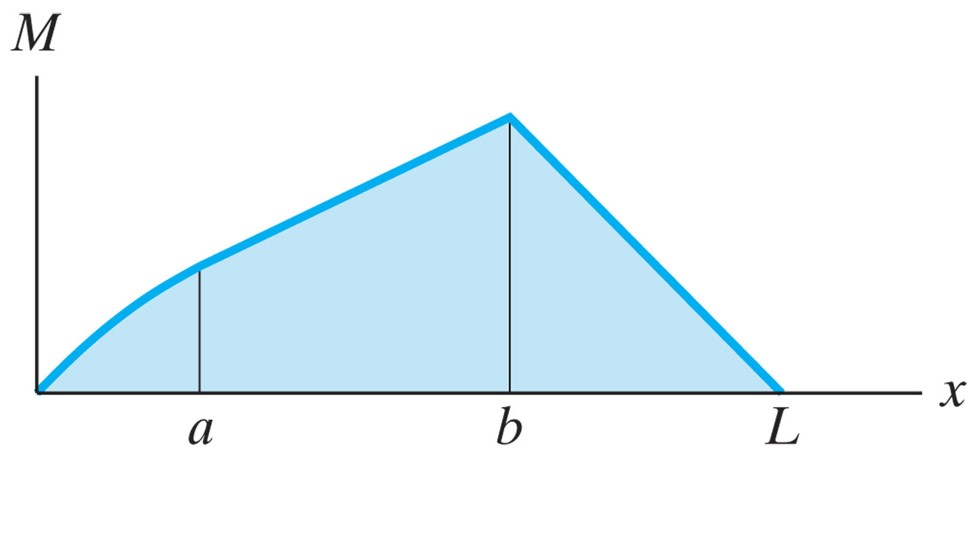
\includegraphics{../images/moment-diagram.jpg}
\end{frame}

\begin{frame}{relation between load, shear, moment}
\protect\hypertarget{relation-between-load-shear-moment}{}
\begin{itemize}
\tightlist
\item
  When there are several forces, supports, or loading conditions applied
  to a beam, the piecewise method can be cumbersome
\item
  In this section we will examine the differential relationships between
  distributed load, shear, and bending moments
\end{itemize}
\end{frame}

\begin{frame}{distributed load}
\protect\hypertarget{distributed-load}{}
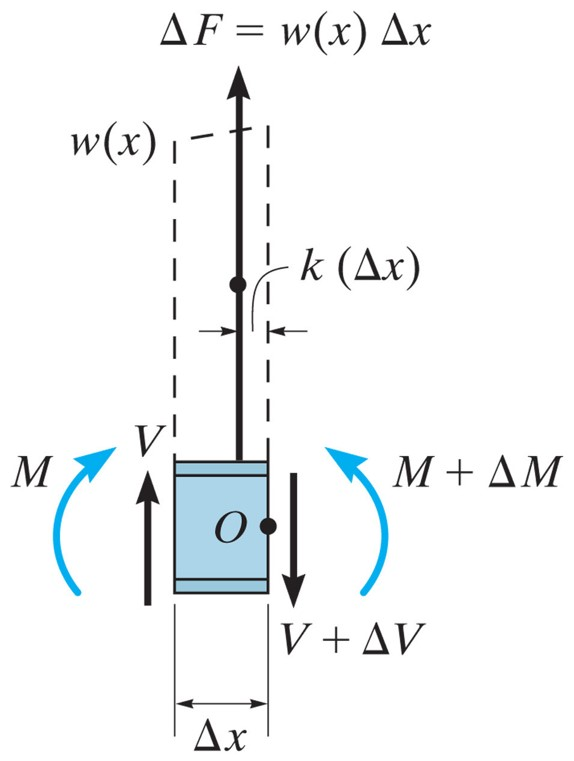
\includegraphics{../images/distributed-load.jpg}
\end{frame}

\begin{frame}{distributed load}
\protect\hypertarget{distributed-load-1}{}
\begin{itemize}
\tightlist
\item
  Consider a beam subjected to only distributed loading
\item
  If we section this beam in the middle (to remove both supports) we can
  relate \emph{V} to the loading function \emph{w}(\emph{x})
\item
  Considering the sum of forces in \emph{y}:
\end{itemize}

\[\begin{aligned}
  V + w(x)\Delta x - (V + \Delta V) &= 0\\
  \Delta V &= w(x) \Delta x
\end{aligned}\]
\end{frame}

\begin{frame}{distributed load}
\protect\hypertarget{distributed-load-2}{}
\begin{itemize}
\tightlist
\item
  If we divide by \(\Delta x\) and let \(\Delta x \to 0\) we find
\end{itemize}

\[\frac{dV}{dx} = w(x)\]

\begin{itemize}
\tightlist
\item
  Thus the slope of the shear diagram is equal to the distributed load
  function
\end{itemize}
\end{frame}

\begin{frame}{moment diagram}
\protect\hypertarget{moment-diagram}{}
\begin{itemize}
\tightlist
\item
  If we consider the sum of moments about \emph{O} on the same section
  we find
\end{itemize}

\[\begin{aligned}
  (M + \Delta M) - (w(x)\Delta x)k \Delta x - V\Delta x - M &= 0\\
  \Delta M &= V \Delta x + k w(x) \Delta x ^2
\end{aligned}\]

\begin{itemize}
\tightlist
\item
  Dividing by \(\Delta x\) and letting \(\Delta x \to 0\) gives
\end{itemize}

\[\frac{dM}{dx} = V\]
\end{frame}

\begin{frame}{concentrated forces}
\protect\hypertarget{concentrated-forces}{}
\begin{itemize}
\tightlist
\item
  If we consider a concentrated force (instead of a distributed load) we
  find
\end{itemize}

\[\Delta V = F \]

\begin{itemize}
\tightlist
\item
  This means that concentrated loads will cause the shear diagram to
  ``jump'' by the amount of the concentrated force (causing a
  discontinuity on our graph)
\end{itemize}
\end{frame}

\begin{frame}{couple moments}
\protect\hypertarget{couple-moments}{}
\begin{itemize}
\tightlist
\item
  If our section includes a couple moment, we find (from the moment
  equation) that
\end{itemize}

\[\Delta M = M_0 \]

\begin{itemize}
\tightlist
\item
  Thus the moment diagram will have a jump discontinuity
\end{itemize}
\end{frame}

\begin{frame}{example 7.9}
\protect\hypertarget{example-7.9}{}
\begin{figure}
\centering
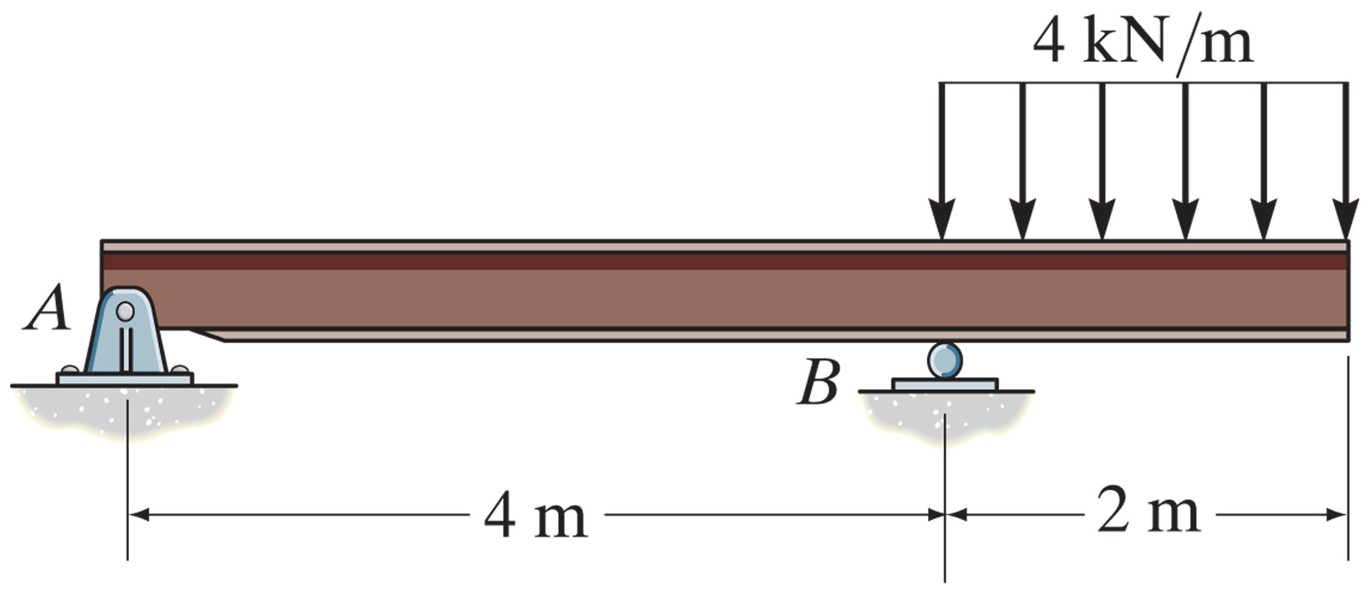
\includegraphics{../images/example-7-9.jpg}
\caption{A beam is 6 meters long with pin supports at the left end, A,
and at B, 4 meters to the right of A. From B to the right end of the
beam is a uniform distributed load of 4 kN/m.}
\end{figure}
\end{frame}

\begin{frame}{example 7.10}
\protect\hypertarget{example-7.10}{}
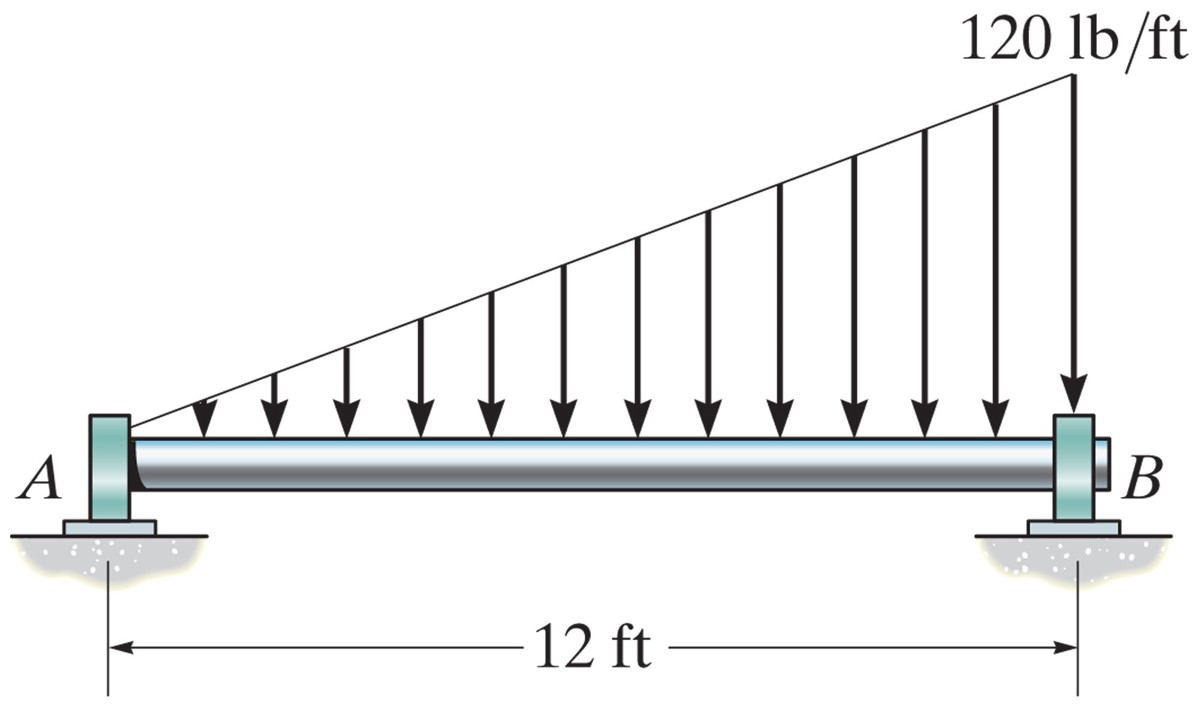
\includegraphics{../images/example-7-10.jpg}
\end{frame}

\begin{frame}{bending deformation}
\protect\hypertarget{bending-deformation}{}
\begin{itemize}
\tightlist
\item
  If we drew a grid on a specimen in bending, we would find that
  vertical lines tend to stay straight (but rotate)
\item
  Horizontal lines will become curved
\item
  If bending lifts the ends up (like a smile), then the top face will be
  in compression (and expand), while the bottom face will be in tension
  (and contract)
\end{itemize}
\end{frame}

\begin{frame}{bending deformation}
\protect\hypertarget{bending-deformation-1}{}
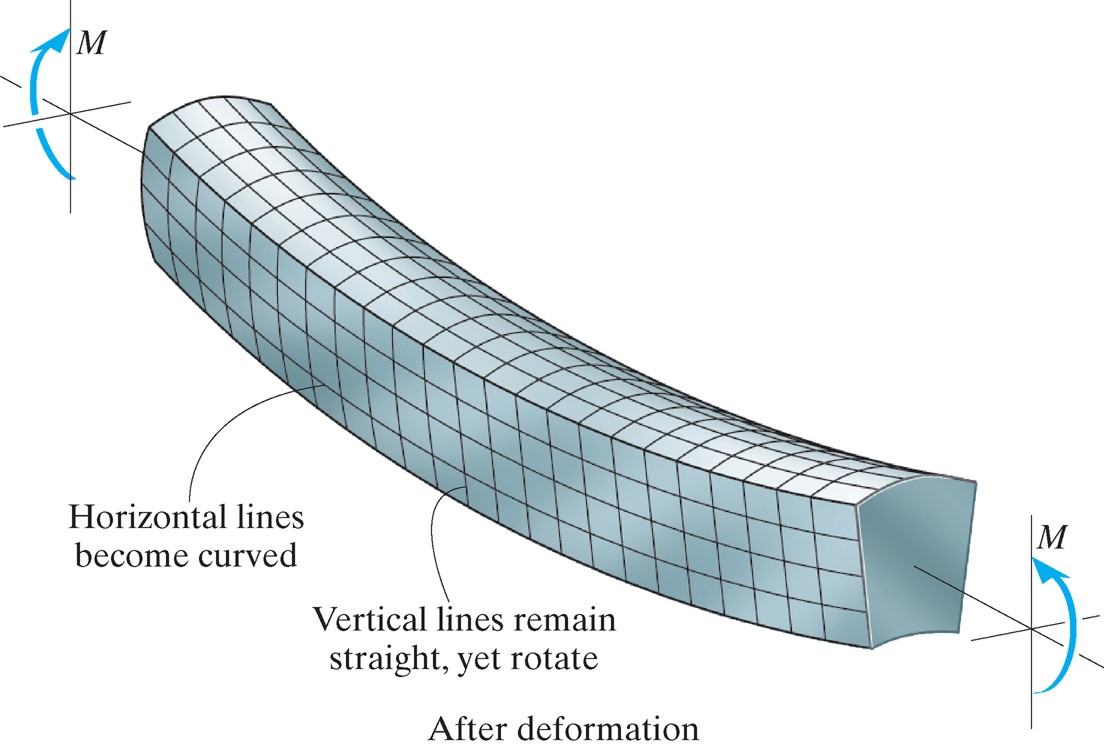
\includegraphics{../images/beam-deformation.jpg}
\end{frame}

\begin{frame}{neutral axis}
\protect\hypertarget{neutral-axis}{}
\begin{itemize}
\tightlist
\item
  Since the bottom is in tension and the top is in compression, there
  must be somewhere in between that is under no stress
\item
  We call that the neutral axis, and assume it does not change in length
\item
  We also assume that planar sections remain planar (no warping)
\item
  Finally, Poisson's effects are neglected (cross-sections keep the same
  size and shape)
\end{itemize}
\end{frame}

\begin{frame}{strain}
\protect\hypertarget{strain}{}
\begin{itemize}
\tightlist
\item
  We will now consider an infinitesimal beam element before and after
  deformation
\item
  \(\Delta x\) is located on the neutral axis and thus does not change
  in length after deformation
\item
  Some other line segment, \(\Delta s\) is located \emph{y} away from
  the neutral axis and changes its length to \(\Delta s ^\prime\) after
  deformation
\end{itemize}
\end{frame}

\begin{frame}{strain}
\protect\hypertarget{strain-1}{}
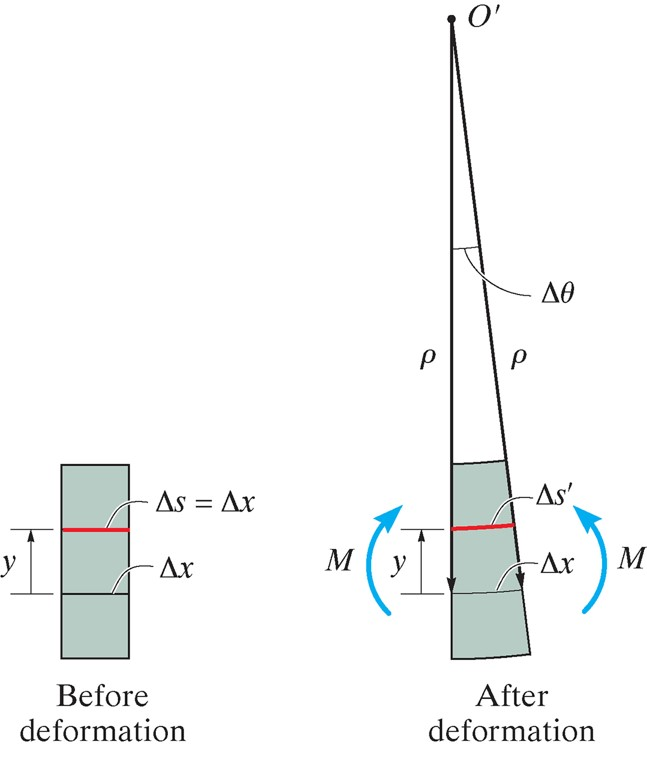
\includegraphics{../images/beam-element.jpg}
\end{frame}

\begin{frame}{strain}
\protect\hypertarget{strain-2}{}
\begin{itemize}
\tightlist
\item
  We can now define strain at the line segment \(\Delta s\) as
\end{itemize}

\[\epsilon = \lim_{\Delta s \to 0} \frac{\Delta s^\prime - \Delta s}{\Delta s}\]
\end{frame}

\begin{frame}{strain}
\protect\hypertarget{strain-3}{}
\begin{itemize}
\tightlist
\item
  If we define \(\rho\) as the radius of curvature after deformation,
  thus \$\Delta x = \Delta s = \rho \Delta \theta \$
\item
  The radius of curvature at \(\Delta s\) is \(\rho - y\), thus we can
  write
\end{itemize}

\[\epsilon = \lim_{\Delta \theta \to 0} \frac{(\rho-y)\Delta \theta - \rho \Delta \theta}{\rho \Delta \theta}\]

\begin{itemize}
\tightlist
\item
  Which gives
\end{itemize}

\[\epsilon = -\frac{y}{\rho}\]
\end{frame}

\begin{frame}{hooke's law}
\protect\hypertarget{hookes-law}{}
\begin{itemize}
\tightlist
\item
  If the beam is a linear material that follows Hooke's Law, the stress
  must be linearly proportional to the strain
\item
  Thus the stress will vary linearly through the beam, just like the
  strain does
\end{itemize}
\end{frame}

\begin{frame}{neutral axis}
\protect\hypertarget{neutral-axis-1}{}
\begin{itemize}
\tightlist
\item
  We have already hypothesized that a neutral axis must exist, we will
  now find its location
\item
  To be in equilibrium, the resultant force(s) produced by the stress
  must sum to zero, which means
\end{itemize}

\[\begin{aligned}
  \sum F_x &= 0 = \int_A dF = \int_A \sigma dA\\
  &= \int_A -\left( \frac{y}{c} \right) \sigma_{max} dA\\
  &= -\frac{\sigma_{max}}{c} \int_A y dA
\end{aligned}\]
\end{frame}

\begin{frame}{neutral axis}
\protect\hypertarget{neutral-axis-2}{}
\begin{itemize}
\tightlist
\item
  Since \(\sigma_{max}\) and \emph{c} are both non-zero constants, we
  know that
\end{itemize}

\[ \int_A y dA = 0\]

\begin{itemize}
\tightlist
\item
  Which can only be satisfied at the horizontal centroidal axis, so the
  neutral axis is the centroidal axis
\end{itemize}
\end{frame}

\begin{frame}{bending moment}
\protect\hypertarget{bending-moment}{}
\begin{itemize}
\tightlist
\item
  The internal bending moment must be equal to the total moment produced
  by the stress distribution
\end{itemize}

\[\begin{aligned}
  M &= \int_A y dF = \int_A y (\sigma dA) \\
  &= \int_A y \left( \frac{y}{c} \sigma_{max} \right) dA \\
  &= \frac{\sigma_{max}}{c} \int_A y^2 dA
\end{aligned}\]
\end{frame}

\begin{frame}{bending moment}
\protect\hypertarget{bending-moment-1}{}
\begin{itemize}
\tightlist
\item
  We recognize that \(\int_A y^2 dA = I\), and we re-arrange to write
\end{itemize}

\[\sigma_{max} = \frac{Mc}{I}\]
\end{frame}

\begin{frame}{procedure}
\protect\hypertarget{procedure}{}
\begin{itemize}
\tightlist
\item
  Find the internal moment at the point of interest, or draw a moment
  diagram to find the maximum point (if needed)
\item
  Determine the moment of inertia for the beam section
\item
  Find the neutral axis and/or the distance from the neutral axis to the
  point of interest
\item
  Use the flexure formula to find the stress
\end{itemize}
\end{frame}

\begin{frame}{example 6.12}
\protect\hypertarget{example-6.12}{}
\begin{figure}
\centering
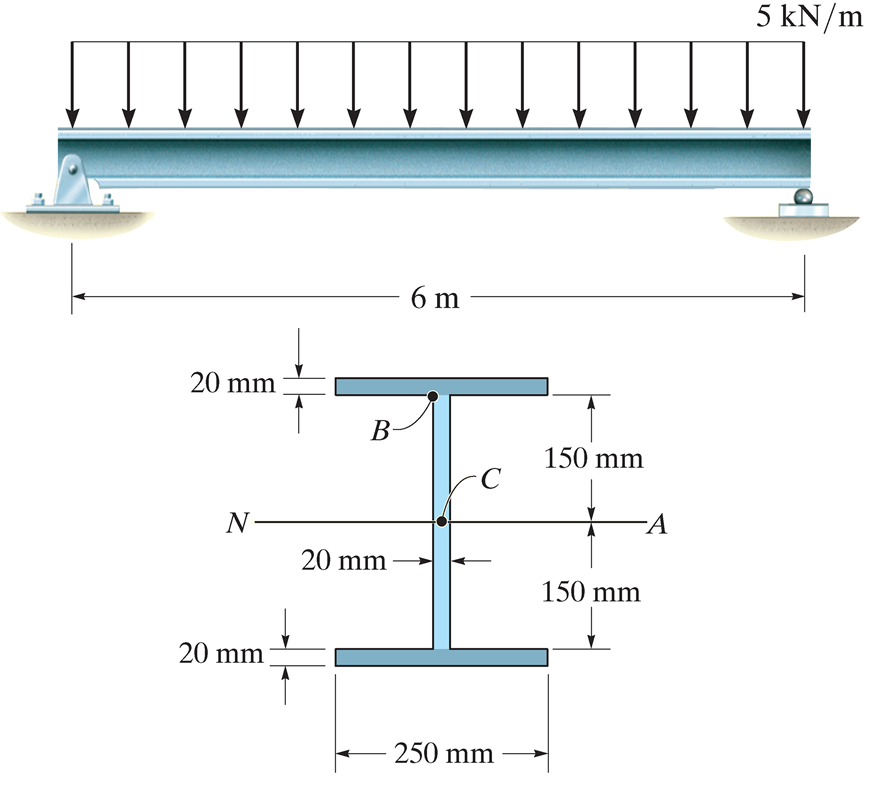
\includegraphics{../images/example-6-12.png}
\caption{A 6 meter long beam is pinned at both ends and subjected to a
uniformly distributed load of 5 kN/m.}
\end{figure}

Find the maximum bending stress and draw the stress distribution through
the thickness at that point.
\end{frame}
